%%%%%%%%%%%%%%%%%%%%%%%%%%%%%%%%%%%%%%%%%%%%%%%%%%%%%%%%%%%%%%%%%%%%%%%%%%%%%%%%%%
\begin{frame}[fragile]\frametitle{}
\begin{center}
{\Large Create Crypto-currency}\\
{\small Ref: Learn with Udemy Courses : Blockchain A-z}
\end{center}
\end{frame}

%%%%%%%%%%%%%%%%%%%%%%%%%%%%%%%%%%%%%%%%%%%%%%%%%%%%%%%%%%%%%%%%%%%%%%%%%%%%%%%%%%
\begin{frame}[fragile]\frametitle{Setup}
\begin{itemize}
\item Additional instillations: requests 2.18.4
\item New file, copy base blockchain code, call file as `your-name coin`
\item Part 1 `Building a Blockchain` remains as is, plus some additions like transactions (ie data) and consensus function.
\item Part 2 `Mining the Blockchain` mostly remains as is
\item Part 3 `Decentralizing Blockchain` gets added newly.
\end{itemize}
\end{frame}

%%%%%%%%%%%%%%%%%%%%%%%%%%%%%%%%%%%%%%%%%%%%%%%%%%%%%%%%%%%%%%%%%%%%%%%%%%%%%%%%%%
\begin{frame}[fragile]\frametitle{Transactions}
\begin{itemize}
\item Transactions are first collected one by one, in blockchain class.
\item Once Miner mines a new block, they get added to it.
\end{itemize}

\begin{lstlisting}
def add_transaction(self, sender, receiver, amount):
		self.transactions.append({'sender': sender,
															'receiver': receiver,
															'amount': amount})
		previous_block = self.get_previous_block() # last block
		return previous_block['index'] + 1 # block index to add these transactions to

\end{lstlisting}
\end{frame}

%%%%%%%%%%%%%%%%%%%%%%%%%%%%%%%%%%%%%%%%%%%%%%%%%%%%%%%%%%%%%%%%%%%%%%%%%%%%%%%%%%
\begin{frame}[fragile]\frametitle{Nodes}
\begin{itemize}
\item Nodes means computers in  the practical world.
\item No particular order, so not stored in `list` but `set`.
\item Each node has address.
\item Parsing is needed to remove `http` etc. an gives the ip in `netloc`. It has port though.
\end{itemize}

\begin{lstlisting}
self.nodes = set() # no particular order

def add_node(self,address):
		parsed_url = urlparse(address)
		self.nodes.add(parsed_url)
\end{lstlisting}
\end{frame}

%%%%%%%%%%%%%%%%%%%%%%%%%%%%%%%%%%%%%%%%%%%%%%%%%%%%%%%%%%%%%%%%%%%%%%%%%%%%%%%%%%
\begin{frame}[fragile]\frametitle{Longest Chain}
\begin{itemize}
\item Look at all nodes (meaning computers)
\item Find the one who has longest chain
\item Here the nodes themselves are stored as urls.
\item Replace any shorter chains with the longest chain.
\end{itemize}

\begin{lstlisting}
def replace_chain(self):
		network = self.nodes
		longest_chain = None
		max_length = len(self.chain)
		for node in network:
				response = requests.get('http://' + node + '/get_chain')
				if response.status_code == 200:
						length = response.json()['length']
						chain = response.json()['chain']
						if length > max_length and self.is_chain_valid(chain):
								max_length = length
								longest_chain = chain
		if longest_chain:
				self.chain = longest_chain
				return True
		return False
\end{lstlisting}
\end{frame}

%%%%%%%%%%%%%%%%%%%%%%%%%%%%%%%%%%%%%%%%%%%%%%%%%%%%%%%%%%%%%%%%%%%%%%%%%%%%%%%%%%
\begin{frame}[fragile]\frametitle{Add Transaction}
\begin{itemize}
\item Usual transactions as well as Miner's fees transactions are added.
\item `uuid4` is used to generate random uuid or address.
\end{itemize}

\begin{lstlisting}
def mine_block():
    :
    blockcahin.add_transaction(sender=node_address,receiver='Yogesh',amount=1)
    block = blockcahin.create_block(proof, previous_hash)
    response = {'message': 'Congrats, you mined a block',
                'index': block['index'],
                'timestamp': block['timestamp'],
                'proof': block['proof'],
                'transactions': block['transactions'],
                'previous_hash': block['previous_hash']}
    return jsonify(response), 200

\end{lstlisting}
\end{frame}

%%%%%%%%%%%%%%%%%%%%%%%%%%%%%%%%%%%%%%%%%%%%%%%%%%%%%%%%%%%%%%%%%%%%%%%%%%%%%%%%%%
\begin{frame}[fragile]\frametitle{Connect Node}
\begin{itemize}
\item New web based POST method to be sent to the blockchain
\item Connect new node to the existing network
\end{itemize}

\begin{lstlisting}
def connect_node():
    json_response = request.get_json()
    nodes = json_response.get('nodes')
    if nodes is None:
        return "No nodes", 400
    for node in nodes:
        blockchain.add_node(node)
    response = {'message': "Added node to network",
                'total_nodes': list(blockchain.nodes)}
    return jsonify(response), 201

\end{lstlisting}
\end{frame}


%%%%%%%%%%%%%%%%%%%%%%%%%%%%%%%%%%%%%%%%%%%%%%%%%%%%%%%%%%%%%%%%%%%%%%%%%%%%%%%%%%
\begin{frame}[fragile]\frametitle{Demo}
\begin{itemize}
\item Make nodes.json with 3 ip addresses, say, just port numbers are different
\item Make transactions.json with 3 fields 'sender','receiver','amount'
\item Make 2 more copies of this py file, so we are all 3, one for each port number
\item Running all 3 apps, one can show transactions between them.
\item Use Postman to send the requests, create 3 tabs in it for each node.
\item First, fire `get\_chain` to see whats there. All 3 will have genesis blocks.
\item Make POST request `connect\_nodes` with `body` (argument) as other two ip addresses than self. Do this for all 3 nodes. No each node is connected with rest of the nodes.
\item Now mine a block on one node. You got one coin as fee.
\item Then fire replace chain, to sync the new block in rest of the nodes
\item Add transactions between nodes and see if they appear fine.
\end{itemize}

\begin{center}
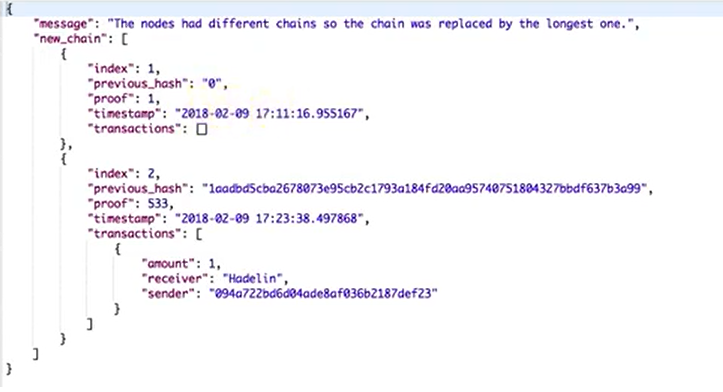
\includegraphics[width=0.4\linewidth,keepaspectratio]{blkchn_27}

{\tiny (Ref:``Blockchain A-Z'' - Udemy)}
\end{center}

\end{frame}


